The data corresponding to sample 8 in Table 6.1 seem unusually large. Remove sample 8.
Construct a joint 95\% confidence region for the mean difference vector $\bm{\delta}$ and the 95\%
Bonferroni simultaneous intervals for the components of the mean difference vector.
Are the results consistent with a test of $H_{0}: \bm{\delta} = \textbf{0}$? Discuss. Does the``outlier'' make a
difference in the analysis of these data?

\begin{figure}[H]
    \centering
    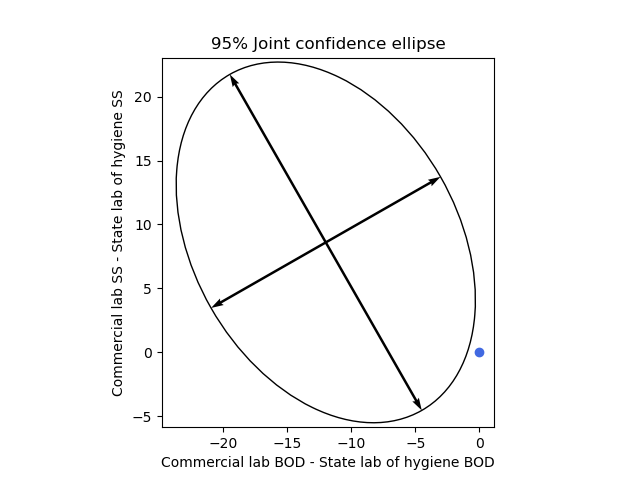
\includegraphics[scale=0.70]{./python/chapter-6/Question-6-3.png}
\end{figure}

This time for Hoteling's $T^{2}$ test $H_{0}: \bm{\delta}^{\prime} = [\delta_{1}, \delta_{2}] = [0, 0] = \textbf{0}^{\prime}$, the zero vector is again not inside the confidence region, so the test would reject.
This doesn't change the conclusion of the $T^{2}$ test found in Example 6.1, but the ellipse did shrink in height and change orientation, where the zero vector is closer to being inside the region.
The other conclusion was that the 95\% simultaneous confidence intervals for $\delta_{1}$ and $\delta_{2}$ did include 0.
This time it looks like $\delta_{1}$ might not include zero, but $\delta_{2}$ still does.

\[
    \bar{d}_{1}
    =
    \frac{ \sum_{j=1}^{n}{ d_{j1} } }{n-1}
    =
    \frac{-120}{10}
    =
    -12
\]
\[
    \bar{d}_{2}
    =
    \frac{ \sum_{j=1}^{n}{ d_{j2} } }{n-1}
    =
    \frac{86}{10}
    =
    8.6
\]
\[
    s_{d_{1}}^{2}
    =
    \frac{ \sum_{j=1}^{n}{( d_{j1} - \bar{d}_{1} )}^{2} }{n-1}
    =
    \frac{1228}{10 - 1}
    =
    136.4444
\]
\[
    s_{d_{2}}^{2}
    =
    \frac{ \sum_{j=1}^{n}{( d_{j2} - \bar{d}_{2} )}^{2} }{n-1}
    =
    \frac{1784.4}{10 - 1}
    =
    198.2667
\]
\[
    t_{n-1}(\alpha/2p)
    =
    t_{11-1}(0.05/[2(2)])
    =
    2.6850
\]
\[
    \delta_{1}:
    \bar{d}_{1}
    \pm
    t_{n - 1}(\alpha)
    \sqrt{ \frac{ s_{d_{1}}^{2} }{n} }
    =
    -12
    \pm
    2.69
    \sqrt{ \frac{ 136.44 }{ 10 } }
    \hspace{0.4cm}\text{or}\hspace{0.4cm}
    (-21.92, -2.08)
\]
\[
    \delta_{2}:
    \bar{d}_{2}
    \pm
    t_{n - 1}(\alpha)
    \sqrt{ \frac{ s_{d_{2}}^{2} }{n} }
    =
    8.6
    \pm
    2.69
    \sqrt{ \frac{ 198.27 }{ 10 } }
    \hspace{0.4cm}\text{or}\hspace{0.4cm}
    (-3.36, 20.56)
\]
The 95\% Bonferroni simultaneous intervals with observation 8 deleted, are a bit different than those with the full data.
Those for $\delta_{1}$, biological oxygen demand (BOD), are pushed more negative and no longer include 0.
Since, both upper and lower bound are negative, there is a significant difference between state and commercial labs, and so, state labs measured higher levels of BOD than commercial labs.
The interval for $\delta_{2}$, suspended solids (SS), has a much lower upper bound, but the lower bound still includes 0.
As we would expect, these intervals are shorter than 95\% simultaneous confidence intervals found on page 277.